% =====================================================================
% STA: Select-Then-Analyze --- arXiv preprint
% Wassim Badraoui --- EPITA / Devoteam --- 2026
% =====================================================================
\documentclass[11pt,a4paper]{article}

\usepackage[utf8]{inputenc}
\usepackage[T1]{fontenc}
\usepackage{lmodern}
\usepackage[english]{babel}

\usepackage[a4paper,margin=2.4cm]{geometry}
\usepackage{setspace}
\setstretch{1.10}

\usepackage{amsmath,amssymb,amsthm,mathtools}
\usepackage{booktabs,array,tabularx}
\usepackage{multirow}
\usepackage{graphicx}
\usepackage[dvipsnames,table]{xcolor}
\usepackage{caption}
\usepackage{subcaption}
\usepackage{tikz}
\usetikzlibrary{arrows.meta,positioning}
\usepackage[hidelinks]{hyperref}
\usepackage{microtype}
\usepackage{authblk}
\usepackage{enumitem}
\setlist{itemsep=0.2em,topsep=0.3em}

\newcommand{\Avg}[1]{\textsc{Avg}@{#1}}
\newcommand{\MRR}{\textsc{MRR}}
\newcommand{\NDCG}[1]{\textsc{NDCG}@{#1}}
\newcommand{\STA}{\textsc{STA}}
\newcommand{\GATv}{\textsc{GATv2}}
\newcommand{\Late}{\textsc{Late-STGCN+GIB}}

\title{\textbf{STA: A Select-Then-Analyze Framework for\\
Scalable Root Cause Analysis in Microservice Architectures}}

\author[1,2]{Wassim Badraoui}
\affil[1]{Devoteam, Paris, France}
\affil[2]{EPITA, Paris, France}
\affil[ ]{\texttt{wassim.badraoui@epita.fr}}

\date{May 2026}

\begin{document}
\maketitle

\begin{abstract}
Root Cause Analysis (RCA) for microservice architectures is dominated by
spatio-temporal Graph Neural Networks (GNNs) operating on the full service
dependency graph, with $O(N^2)$ spatial cost. As production meshes grow past
50--100 services this cost becomes prohibitive for sub-second incident
response. We present \STA{} (\emph{Select-Then-Analyze}), an early-bottleneck
spatio-temporal GNN that reduces RCA complexity to $O(N + k^{2})$ by selecting
a compact candidate subgraph of $k \ll N$ nodes before any deep spatial
analysis. Selection is performed by a Straight-Through Estimator with annealed
Gumbel noise, regularized by a Variational Graph Information Bottleneck loss
that is \emph{asymmetric} between healthy and faulty windows. We evaluate four
model variants (\STA{}, \GATv{}, and their multimodal extensions) under a single
shared protocol of 5 deterministic seeds across four regimes: (i)~Barab\'asi--Albert
synthetic graphs at $N\in\{20,50,100\}$; (ii)~three RCAEval public benchmarks
(TrainTicket, SockShop, Online Boutique); (iii)~a live 14-service sock-shop
deployment on a private Kubernetes cluster with Chaos Mesh fault injection
(metrics-only and metrics+logs); and (iv)~a 50-service synthetic-but-real
deployment on the same cluster. Three results are reported and explicitly
scoped. First, \STA{}'s asymptotic advantage transfers from simulation to real
clusters: $+5.8$ percentage points (pp) \Avg{1} over \GATv{} at $N{=}50$ on
the cluster, with $4.6\times$ lower variance. Second, at small graph scale
$(N{\le}14)$ \STA{} and \GATv{} are within the noise envelope of five-seed
evaluation. Third, multimodal fusion on RCAEval degrades or matches
metrics-only performance on TrainTicket and Online Boutique ($-5{-}14$ pp
\Avg{1}), while on the same cluster it leaves \Avg{1} unchanged but
\emph{halves} seed-to-seed variance ($\sigma\!:\!4.3 \to 2.1$). Beyond
evaluation, we contribute an end-to-end pipeline: 25-trial Optuna HPO,
self-describing model bundle, FastAPI inference service with Prometheus
metrics, ADWIN drift detector with cooldown, and a four-mechanism gray-failure
detector whose synthetic A/B raises gray \Avg{1} from $0.602$ to $1.000$ at
zero cost on hard and cascade scenarios. We do not claim SOTA; we ship an
explicit comparability matrix flagging \emph{partially comparable} vs.
\emph{not isoperimeter} verdicts for every published baseline. All code,
manifests, SHA-256-pinned result JSONs and Docker artifacts are released at
\url{https://github.com/Wassbdr/matrix_simple}.
\end{abstract}

\section{Introduction}
\label{sec:intro}

Modern cloud-native applications deploy business logic across tens to hundreds
of loosely coupled microservices. When an incident occurs, identifying the
\emph{root cause} (RC) service---the node that first entered a faulty
state---is the prerequisite for any automated remediation. In production
environments with dozens of instrumented services, manual triage routinely
takes tens of minutes, creating direct business impact.

RCA for microservices is hard for three reasons.
\textbf{(i)~Failures propagate}: a single faulty service sends error signals
upstream to its callers, causing a cascade of symptomatic anomalies that
masks the original cause. \textbf{(ii)~Signals are heterogeneous}: the
observable evidence spans time-series metrics, unstructured logs, and
distributed traces, each modality carrying partially overlapping but distinct
information. \textbf{(iii)~The search space grows}: at $N{=}100$ services, a
naive pairwise spatial convolution costs $O(N^2)\!=\!10{,}000$ operations per
layer; at $N{=}500$ this becomes prohibitive for sub-second diagnosis.

GNN approaches operating on the service dependency graph have shown strong
performance on small public benchmarks ($N\!=\!5$), with architectures ranging
from full-graph GCNs to attention-based spatio-temporal models. However,
several questions remain under-explored:

\begin{enumerate}
  \item \textbf{Scalability.} Does the spatial bottleneck in full-graph GNNs
  limit their practical deployment at large $N$? Can a principled selection
  step reduce this cost without sacrificing recall?
  \item \textbf{Graph vs.\ temporal.} At the small-$N$ scale of public
  benchmarks, does graph structure actually help over a pure temporal encoder,
  or does it inject noise?
  \item \textbf{Multimodal integration.} Do logs and traces complement
  metrics, or do they introduce gradient conflicts that net-hurt performance?
  \item \textbf{Operational robustness.} How do RCA models behave during
  Kubernetes rolling updates (concept drift) and under \emph{gray}
  failures---anomalies that stay below per-metric SLO thresholds yet degrade
  system performance?
\end{enumerate}

This paper makes four contributions.

\textbf{C1.~\STA{} (Section~\ref{sec:sta}).} An early-bottleneck spatio-temporal
GNN that achieves $O(N + k^{2})$ inference via differentiable top-$k$ node
selection with annealed Gumbel noise and a Straight-Through Estimator. A
Variational GIB regularizer is used in place of an $L_1$ sparsity penalty
and is \emph{asymmetric} between healthy and faulty windows.

\textbf{C2.~Systematic multi-regime evaluation (Sections~\ref{sec:proto},
\ref{sec:results}).} Four model variants are benchmarked across simulated
Barab\'asi--Albert graphs at $N \in \{20,50,100\}$, three RCAEval datasets, a
live 14-service Kubernetes cluster, and a 50-service synthetic-but-real
deployment on the same cluster. \Avg{k}, \MRR{}, and \NDCG{3} are reported
with standard deviations across five independent seeds. Every JSON artifact
is SHA-256-pinned.

\textbf{C3.~A robust negative result on multimodal fusion
(Section~\ref{sec:mm}).} Adding logs and traces to metrics degrades or matches
metrics-only performance on RCAEval, while leaving \Avg{1} unchanged but
halving variance on the live cluster. Three explanatory hypotheses are
proposed.

\textbf{C4.~An operational stack (Section~\ref{sec:ops}).} ADWIN-based
concept-drift detector with per-metric cooldown; a four-mechanism composite
gray-failure detector (P99/P50 micro-stutter, inter-metric decorrelation,
Mann--Kendall trend, Limplock); a Variational GIB loss; three variants of a
cascade-aware loss including a learnable propagation matrix; a 25-trial
Optuna HPO loop; a self-describing model bundle; and a FastAPI inference
service with Prometheus metrics deployed on the same private cluster.

We \emph{do not} claim state-of-the-art. Section~\ref{sec:comparability}
ships an explicit comparability matrix that classifies every baseline
comparison as \emph{partially comparable} (metrics-only) or \emph{not
isoperimeter} (multimodal). All numbers in this paper are reproducible from
the released code, datasets, and seeds.

\section{Related Work}
\label{sec:related}

\textbf{RCA for microservices.} Early systems rely on correlation-based
propagation. MicroRCA~\cite{wu2020microrca} constructs a weighted service
graph from Pearson correlations and applies random walks; CausaRank refines
this with a causal ranking formulation; E-Diagnosis~\cite{shan2019ediagnosis}
introduces disentangled representation learning; BARO~\cite{pham2024baro} uses
bootstrap anomaly ranking and is the strongest reproduced baseline. The
RCAEval benchmark~\cite{pham2024rcaeval} provides reference implementations
and reported numbers for the four baselines above on TrainTicket, SockShop,
Online Boutique, and other systems. We compare against the RCAEval reference
numbers and explicitly qualify the comparison
(Section~\ref{sec:comparability}).

\textbf{GNN-based fault localization.} Spatio-temporal GNNs have shown strong
performance on traffic prediction (STGCN~\cite{yu2018stgcn}). The Information
Bottleneck~\cite{tishby2015ib} and its graph adaptation
GIB~\cite{wu2020gib} provide a principled framework for sparse graph
representations by maximizing $I(Z;Y)$ while minimizing $I(Z;X)$. Prior work
applies GIB at the graph level; we adapt it to \emph{node-level} mask
learning for selective subgraph extraction.
GATv2~\cite{brody2022gatv2} fixes the static-attention limitation of the
original GAT~\cite{velickovic2018gat} by applying the linear projection to the
concatenation of source and target features \emph{before} the nonlinearity.

\textbf{Multimodal fault diagnosis.} The intuition is that metrics, logs and
traces capture complementary aspects of system health. The literature
commonly assumes that fusion improves over any one modality. We show on
RCAEval that, when log/trace coverage is sparse or low-signal, fusion
introduces optimization interference~\cite{yu2020gradsurg} and net-hurts
\Avg{1}.

\textbf{Gray failures and drift.} Gray failures~\cite{huang2017gray} are
partial failures where individual metrics remain within their alert
thresholds while the system is degraded. Two patterns are particularly
relevant: metastable degraded states and ``limplock'' (saturation under
apparent idleness). Our detector targets these explicitly
(Section~\ref{sec:ops}). For drift, we adapt
ADWIN~\cite{bifet2007adwin} with per-metric cooldown to suppress RCA output
during Kubernetes rolling updates.

\section{Problem Formulation}
\label{sec:formulation}

We model a microservice system as a directed graph $G = (V, E)$ with
$V = \{v_1, \dots, v_N\}$ services and edges $E \subseteq V \times V$ encoding
runtime call dependencies. Each service $v_i$ is observed through a
multivariate time series $X_i \in \mathbb{R}^{T \times F}$ where $T$ is the
window length and $F$ the per-service metric count. The full system
observation is $X \in \mathbb{R}^{T \times N \times F}$.

We define three fault taxonomy classes:
\textbf{Hard failures}---the RC service exhibits a sharp, isolated anomaly
(CPU spike, OOM kill, pod termination); signal is strong and localized.
\textbf{Cascade failures}---a fault at $v_{rc}$ propagates over multiple hops,
generating secondary symptoms downstream.
\textbf{Gray failures}---all per-service metrics remain within SLA, yet joint
behavior degrades, detectable only through inter-metric decorrelation or
subtle trend analysis.

We treat fault localization as a sparse inverse problem: a perturbation
$U \in \mathbb{R}^N$ is applied to the system dynamics, and the learner must
recover $\mathrm{supp}(U)$ from $X$. In the single-fault regime
$\lVert U \rVert_0 = 1$, the model produces a ranked list of candidate root
causes and is scored by $\Avg{k}$, $\MRR{}$, and $\NDCG{k}$.

\section{Method: \STA{}}
\label{sec:sta}

\subsection{Architecture}
\STA{} processes an input window in five stages
(Fig.~\ref{fig:sta-pipeline}). The cost of each stage is given alongside.

\paragraph{Stage 1 ($O(N)$): LightEncoder.}
For each node independently (no message passing yet), a stack of two 1D
temporal convolutions followed by a temporal attention pooling produces a
node embedding $h_i \in \mathbb{R}^H$ from $X_i \in \mathbb{R}^{T \times F}$:
\begin{align}
  h_i^{(1)} &= \mathrm{ReLU}(\mathrm{Conv1d}(X_i; k{=}3)), \\
  h_i^{(2)} &= \mathrm{ReLU}(\mathrm{Conv1d}(h_i^{(1)}; k{=}3)), \\
  \alpha_i  &= \mathrm{softmax}_t\big(W_\alpha \tanh(W_q h_i^{(2)})\big), \\
  h_i       &= \textstyle\sum_t \alpha_i^t \, h_i^{(2),t}.
\end{align}
The zero-hop constraint is deliberate: applying graph convolution before
selection causes over-smoothing~\cite{li2018smoothing} at large $N$, blending
node representations and reducing the discriminability of individual fault
signatures. The selector must see local node features, not
neighborhood-averaged ones.

\paragraph{Stage 2 ($O(N)$): STESelector.}
A small MLP $g_\theta$ computes per-node logits and adds Gumbel noise with
temperature $\tau$, then a soft sigmoid mask is hardened by a top-$k$
operation:
\begin{align}
  s_i &= g_\theta(h_i) + \mathrm{Gumbel}(0, \beta), \\
  M_{\mathrm{soft},i} &= \sigma(s_i / \tau), \\
  M_{\mathrm{hard}}   &= \mathrm{TopK}(M_{\mathrm{soft}}, k), \\
  M_{\mathrm{STE}}    &= M_{\mathrm{hard}} + M_{\mathrm{soft}} - \mathrm{sg}(M_{\mathrm{soft}}). \label{eq:ste}
\end{align}
The annealed temperature $\tau$ prevents premature collapse to a
deterministic top-$k$; the Straight-Through
Estimator~\cite{bengio2013ste,jang2017gumbel} routes gradients through
$M_{\mathrm{soft}}$ during the backward pass while the forward pass uses
$M_{\mathrm{hard}}$.

\paragraph{Stage 3 ($O(E)$): Subgraph extraction.}
A single vectorized \texttt{pyg\_subgraph} call extracts the induced
subgraph $S = G[\,\mathrm{supp}(M_{\mathrm{hard}})\,]$.

\paragraph{Stage 4 ($O(k^{2})$): DeepSTGCN.}
Two 1D temporal convolutions followed by two
GCN~\cite{kipf2017gcn} layers, applied \emph{exclusively} on the $k$-node
subgraph:
\begin{equation}
  H_{\mathrm{gcn}} = \mathrm{GCN}\big(\mathrm{GCN}(\mathrm{Conv1d}_2(X_S), A_S), A_S\big).
\end{equation}

\paragraph{Stage 5 ($O(k)$): SubgraphScorer with residual blend.}
\begin{equation}
  \ell = (1-\alpha)\cdot\mathrm{MLP}_{\mathrm{score}}(H_{\mathrm{gcn}})
       + \alpha \cdot s_{\mathrm{selected}}, \label{eq:blend}
\end{equation}
where $\alpha \in [0,1]$ is a learnable scalar. Unselected nodes receive
$\ell = -\infty$. The residual constraint lets the deep analyzer refine---but
not contradict---the selector's initial ranking.

\begin{figure}[t]
\centering
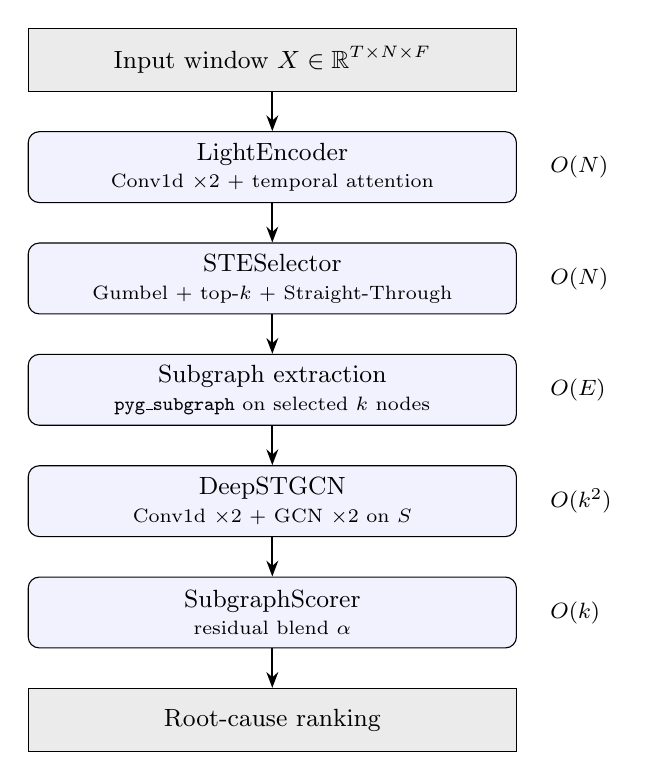
\begin{tikzpicture}[
  node distance=5mm,
  box/.style={draw, rounded corners, align=center, font=\small,
              minimum width=62mm, minimum height=9mm, fill=blue!5},
  io/.style={draw, align=center, font=\small, minimum width=62mm,
             minimum height=8mm, fill=black!8},
  cmplx/.style={font=\footnotesize\itshape, anchor=west},
  arr/.style={-{Stealth[length=2mm]}, thick}]
  \node[io] (x) {Input window $X \in \mathbb{R}^{T\times N\times F}$};
  \node[box, below=of x]    (enc)   {LightEncoder\\[-1pt]{\scriptsize Conv1d $\times2$ + temporal attention}};
  \node[box, below=of enc]  (sel)   {STESelector\\[-1pt]{\scriptsize Gumbel + top-$k$ + Straight-Through}};
  \node[box, below=of sel]  (sub)   {Subgraph extraction\\[-1pt]{\scriptsize \texttt{pyg\_subgraph} on selected $k$ nodes}};
  \node[box, below=of sub]  (deep)  {DeepSTGCN\\[-1pt]{\scriptsize Conv1d $\times2$ + GCN $\times2$ on $S$}};
  \node[box, below=of deep] (score) {SubgraphScorer\\[-1pt]{\scriptsize residual blend $\alpha$}};
  \node[io, below=of score] (out)   {Root-cause ranking};
  \foreach \a/\b in {x/enc, enc/sel, sel/sub, sub/deep, deep/score, score/out}
    \draw[arr] (\a) -- (\b);
  \node[cmplx, right=3mm of enc]   {$O(N)$};
  \node[cmplx, right=3mm of sel]   {$O(N)$};
  \node[cmplx, right=3mm of sub]   {$O(E)$};
  \node[cmplx, right=3mm of deep]  {$O(k^2)$};
  \node[cmplx, right=3mm of score] {$O(k)$};
\end{tikzpicture}
\caption{\STA{} five-stage pipeline. The early bottleneck (STESelector) caps the
deep spatial analysis at $k \ll N$ nodes, yielding $O(N+k^{2})$ per forward pass
instead of the $O(N^2)$ of full-graph models.}
\label{fig:sta-pipeline}
\end{figure}

\subsection{Asymmetric Variational GIB Loss}
\label{sec:vgib}

Rather than an $L_1$ penalty on $M_{\mathrm{soft}}$ that uniformly drives the
mask towards sparsity, we use a Variational GIB regularizer that is
\emph{asymmetric} between healthy and anomalous windows:
\begin{align}
  \mathcal{L}_{\mathrm{healthy}}    &= \mathbb{E}\big[\,M_{\mathrm{soft}}^{2}\,\big], \\
  \mathcal{L}_{\mathrm{anomalous}}  &= -\mathrm{Entropy}(M_{\mathrm{soft}})
                                       + \big\lVert \tfrac{1}{N}\mathbf{1} - \overline{M_{\mathrm{soft}}}\big\rVert^{2}.
\end{align}
On healthy windows the loss pushes the mask to zero (no RC active, reduces
false positives); on anomalous windows it encourages a concentrated, near
one-hot mask (improving \Avg{1} over $L_1$). The total training loss is
\begin{equation}
  \mathcal{L} = \mathcal{L}_{\mathrm{CE}}
              + \lambda_{\mathrm{NCE}} \mathcal{L}_{\mathrm{InfoNCE}}
              + \lambda_{\mathrm{GIB}} \mathcal{L}_{\mathrm{GIB}}
              + \lambda_{\mathrm{c}}   \mathcal{L}_{\mathrm{cascade}},
\end{equation}
where $\mathcal{L}_{\mathrm{cascade}}$ enforces structural distance-proportional
score gaps (Section~\ref{sec:cascade}).

\subsection{Baselines and Variants}
\label{sec:baselines}

\textbf{\GATv{} (Late Bottleneck).} Two GATv2~\cite{brody2022gatv2} layers
process the full graph, and node importance is read off as the sum of
incoming attention weights:
$\text{imp}_i = \sum_{j:(j,i)\in E}\alpha_{ji}$; $\ell_i = \mathrm{MLP}(H_{\mathrm{gat2}})_i + \beta\,\text{imp}_i$.
Soft attention spreads weight along cascade chains, making \GATv{} a natural
counterpart to \STA{}'s hard top-$k$ on multi-hop scenarios.

\textbf{\Late{}.} A late-bottleneck GCN with a GIB mask applied \emph{after}
two GCN layers, providing a third reference point.

\textbf{\STA{}-MM and \GATv{}-MM.} Multimodal extensions with three
modality-specific encoders (metrics: Conv1d; logs: MLP + LayerNorm; traces:
MLP + LayerNorm), fused either via cross-modal mask attention (\STA{}-MM) or
late feature concatenation (\GATv{}-MM). Missing modalities collapse to
uniform contributions.

\section{Pipeline Components}
\label{sec:ops}

\paragraph{Cascade-Aware Loss.}
\label{sec:cascade}
Three variants enforce distance-proportional score gaps between the RC and
downstream cascade nodes. The \emph{structural} variant applies hinge
constraints on graph hop distance with margins $0.5$ (1-hop) and $0.3$
(2-hop). The \emph{causal-weighted} variant scales margins by causal edge
weights. The \emph{learnable} variant trains a full $N{\times}N$ propagation
matrix $B$ jointly with the model.

\paragraph{ADWIN Drift Detector.}
We monitor all $F{=}6$ Prometheus metrics per service with
ADWIN~\cite{bifet2007adwin}. Drift is declared when more than $50\%$ of
metrics simultaneously trigger; a 30-timestep cooldown then suppresses RCA
output to prevent false positives during Kubernetes rolling updates and
cold starts.

\paragraph{Four-mechanism Gray Failure Detector.}
Triggered in priority order:
(i)~\textbf{P99/P50 micro-stutter}: ratio $\!>\!3.0$ flags tail-latency
amplification from CPU steal or GC pauses;
(ii)~\textbf{Inter-metric decorrelation}: mean pairwise Pearson drop
$\!>\!0.4$ relative to a rolling baseline;
(iii)~\textbf{Mann--Kendall trend}~\cite{mann1945mk}: $|S/S_{\max}|\!>\!0.6$
targets nascent metastable degradation;
(iv)~\textbf{Limplock}: $q_{\mathrm{rate}}/u_{\mathrm{cpu}}\!>\!5.0$ detects
saturation under idleness.
Triggered nodes receive a score boost ($\times 3$) before final ranking.

\paragraph{Causal Graph Builder.}
A cascade of causal discovery algorithms with automatic fallback:
PC~\cite{spirtes2000causation} (Fisher's $z$, $\alpha\!=\!0.05$)
$\rightarrow$ FCI (latent confounders)
$\rightarrow$ Granger~\cite{granger1969} (lags 1--3)
$\rightarrow$ structural BA edges as default. The final graph is the weighted
union of discovered causal edges (weight $2.0$) and structural edges
(weight~$1.0$).

\paragraph{HPO, Bundle, Serving.}
A 25-trial Optuna study on the sock-shop windows (seed $42$) optimizes
$\MRR{}$; the best configuration is retrained over $5$ seeds and serialized
into a self-describing bundle (\texttt{state\_dict} + scaler + metadata
+ HPO provenance). The bundle is loaded by a FastAPI inference service
exposing \texttt{/predict}, \texttt{/health}, \texttt{/ready},
\texttt{/info}, \texttt{/metrics}, and is deployed on the same private
Kubernetes cluster.

\section{Experimental Protocol}
\label{sec:proto}

\subsection{Datasets}

\textbf{Synthetic BA graphs.} Scale-free random graphs with
$N \in \{20, 50, 100\}$ and connectivity $m{=}2$, generated by preferential
attachment. About 3{,}000 windows per configuration with balanced
hard/cascade/gray fault types and a $20\%$ healthy-window ratio.

\textbf{RCAEval (public, $N{=}5$).} Three Kubernetes microservice systems
shipped with the benchmark~\cite{pham2024rcaeval}: TrainTicket (Java),
SockShop (Go), Online Boutique (polyglot). Faults from Chaos Mesh
(CPU/memory stress, network delay/loss, pod kill); 90 scenarios per dataset
in our evaluation slice.

\textbf{ObservIT live cluster, sock-shop, $N{=}14$.} Five chaos manifests
(Table~\ref{tab:scenarios}) covering all three fault classes. Five Locust
load profiles. Prometheus + Loki + Jaeger collection. The full campaign
runs via \texttt{scripts/run\_sockshop\_campaign.sh}.

\textbf{ObservIT live cluster, massive, $N{=}50$.} A synthetic-but-real
deployment of 50 dummy services on the same cluster, generated from a
BA-like topology JSON shipped under \texttt{rca\_pipeline/k8s\_massive/}.
This keeps the K8s deployment and the GNN edge index strictly aligned:
\texttt{topologies.py} loads the JSON and registers a \texttt{massive\_n50}
topology entry which \texttt{benchmark\_real.py} accepts directly via the
\texttt{--observit-topology} flag.

\begin{table}[t]
\centering\small
\begin{tabularx}{\linewidth}{lXll}
\toprule
\textbf{Scenario} & \textbf{Mechanism} & \textbf{Type} & \textbf{RC} \\
\midrule
\texttt{stress-cpu-catalogue}        & CPU stress workers @ 80\% & hard & catalogue \\
\texttt{stress-mem-carts}            & 256\,MB memory allocation & hard & carts \\
\texttt{network-delay-orders-orders-db} & 400\,ms latency, 80\,ms jitter & cascade & orders-db \\
\texttt{network-loss-catalogue-db}   & 15\,\% packet loss & gray & catalogue-db \\
\texttt{pod-kill-user}               & periodic pod termination & hard & user \\
\bottomrule
\end{tabularx}
\caption{Five chaos scenarios injected on the live sock-shop cluster.}
\label{tab:scenarios}
\end{table}

\subsection{Protocol}

All experiments use five seeds: $\{42, 123, 7, 1337, 2025\}$ (three for the
$N{=}50$ cluster, due to per-seed campaign time). For each seed a distinct
stratified train/test split is produced (\texttt{train\_ratio=0.8},
\texttt{varying\_split\_by\_run\_seed} mode), so the reported variances
reflect both initialization variance and split variance. Training:
100 epochs (real), 150 epochs (synthetic) plus 80 epochs of contrastive
pre-training for the \Late{} family. Hidden $H{=}32$; Adam
($\text{lr}{=}10^{-3}$, $\text{wd}{=}10^{-4}$); batch 256. All real-data runs
enforce \texttt{--sta-contrastive-warmup 0}: warmup destabilizes \STA{} on
real datasets by overfitting to within-dataset topology biases.

\paragraph{Statistical disclaimer.} With $n{=}5$ seeds, bootstrap-based
$95\%$ CIs and formal significance tests are not statistically reliable;
every JSON includes a \texttt{seed\_level\_bootstrap\_reliable: false} flag.
We therefore report mean $\pm$ one standard deviation across seeds and treat
a difference as \emph{meaningful} only when it exceeds the larger of the two
standard deviations; otherwise we mark it \emph{within noise}.

\subsection{Comparability Matrix}
\label{sec:comparability}

The published RCAEval baselines (BARO, E-Diagnosis, CausaRank, MicroRCA) are
reproduced from the RCAEval reference numbers shipped with the benchmark.
Their split strategy, number of seeds, case filtering, and preprocessing are
not fully specified. We therefore classify our baseline comparisons as
\emph{partially comparable} for metrics-only evaluations and \emph{not
isoperimeter} for multimodal evaluations. When our \Avg{1} exceeds a published
baseline, we cannot rule out a protocol-difference confound. To remove that
confound for the strongest baseline, we additionally re-implement BARO under
our \emph{exact} protocol --- same cases, candidate node set, per-seed split and
metric functions (Section~\ref{sec:results}, Table~\ref{tab:baro-iso}). Under
identical conditions BARO is markedly stronger than its published number and our
models do \emph{not} uniformly beat it; we make no SOTA claim.

\section{Results}
\label{sec:results}

\subsection{Synthetic BA Graphs --- Scaling}

\begin{table}[t]
\centering\small
\begin{tabular}{lcccc}
\toprule
\textbf{Model} & $N{=}20$ & $N{=}50$ & $N{=}100$ & $N{=}100$ latency (ms) \\
\midrule
\STA{}            & $80.5 \pm 12.2$ & $58.9 \pm 4.9$  & $\mathbf{55.2 \pm 4.6}$ & $3.4 \pm 0.8$ \\
\GATv{}           & $82.8 \pm 3.9$  & $\mathbf{57.1 \pm 2.3}$ & $49.0 \pm 2.9$ & $3.0 \pm 1.3$ \\
\Late{}           & $82.3 \pm 4.7$  & $46.9 \pm 6.8$  & $47.1 \pm 9.7$ & $2.5 \pm 1.4$ \\
Full-Graph GCN    & $\mathbf{83.0 \pm 2.9}$ & $52.6 \pm 2.6$ & $46.6 \pm 4.2$ & $1.8 \pm 0.4$ \\
Random Forest     & $68.5 \pm 2.7$  & $31.2 \pm 1.6$  & $\phantom{0}6.5 \pm 0.9$ & n/a \\
MLP               & $\phantom{0}8.4 \pm 2.4$ & $\phantom{0}2.9 \pm 0.5$ & $\phantom{0}1.1 \pm 0.4$ & n/a \\
\bottomrule
\end{tabular}
\caption{Synthetic BA, $\Avg{1}\,(\%)\pm\sigma$ over 5 seeds. \STA{} leads at
$N{=}100$ by $+6{-}9$ pp over $O(N^2)$ full-graph models while keeping
inference under $3.5$~ms.}
\label{tab:sim}
\end{table}

\begin{figure}[t]
\centering
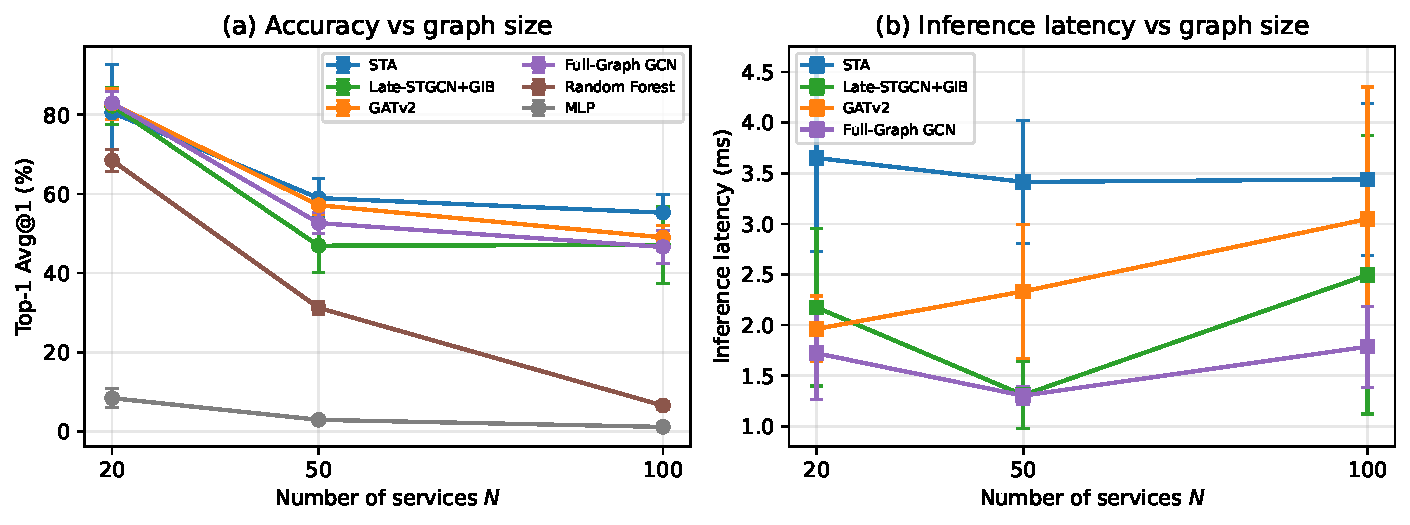
\includegraphics[width=\linewidth]{figures/scaling.pdf}
\caption{Scaling on synthetic BA graphs (5 seeds, $\pm\sigma$).
(a)~\STA{} is the only model whose \Avg{1} lead grows with $N$;
(b)~\STA{}'s per-query latency stays flat (bounded by $O(k^2)$) while
attention/full-graph models trend upward with $N$.}
\label{fig:scaling}
\end{figure}

Table~\ref{tab:sim} shows that the four GNN models are statistically tied at
$N{=}20$ (within noise envelope). At $N{=}50$, the three Late/Full models
degrade by $\sim 30$ pp; \STA{} retains a $+1.8$ pp lead over \GATv{}. At
$N{=}100$, \STA{} extends this lead to $+6.2$ pp over \GATv{}, $+8.1$ pp
over \Late{}, and $+8.6$ pp over the Full-Graph GCN, while inference cost
stays below $3.5$~ms. Crucially, \STA{} is the only model that does
\emph{not} collapse on the cheap baselines as $N$ grows---Random Forest
drops to $6.5\%$ and MLP to $1.1\%$ at $N{=}100$.

\subsection{RCAEval --- Metrics-Only, $N{=}5$}

\begin{table}[t]
\centering\small
\begin{tabular}{lcccc}
\toprule
\textbf{Dataset} & \STA{} \Avg{1} & \STA{} \MRR{} & \GATv{} \Avg{1} & \GATv{} \MRR{} \\
\midrule
TrainTicket      & $\mathbf{96.0 \pm 3.7}$  & $\mathbf{98.0 \pm 1.9}$  & $95.0 \pm 4.5$ & $97.5 \pm 2.2$ \\
SockShop         & $\mathbf{85.0 \pm 8.9}$  & $\mathbf{90.8 \pm 5.8}$  & $81.0 \pm 8.0$ & $87.6 \pm 5.8$ \\
Online Boutique  & $65.0 \pm 9.5$           & $77.9 \pm 5.3$           & $\mathbf{68.0 \pm 5.1}$ & $\mathbf{78.8 \pm 4.2}$ \\
\bottomrule
\end{tabular}
\caption{RCAEval metrics-only, $\Avg{1}/\MRR{}\,(\%)\pm\sigma$, 5 seeds.}
\label{tab:rcaeval}
\end{table}

\begin{figure}[t]
\centering
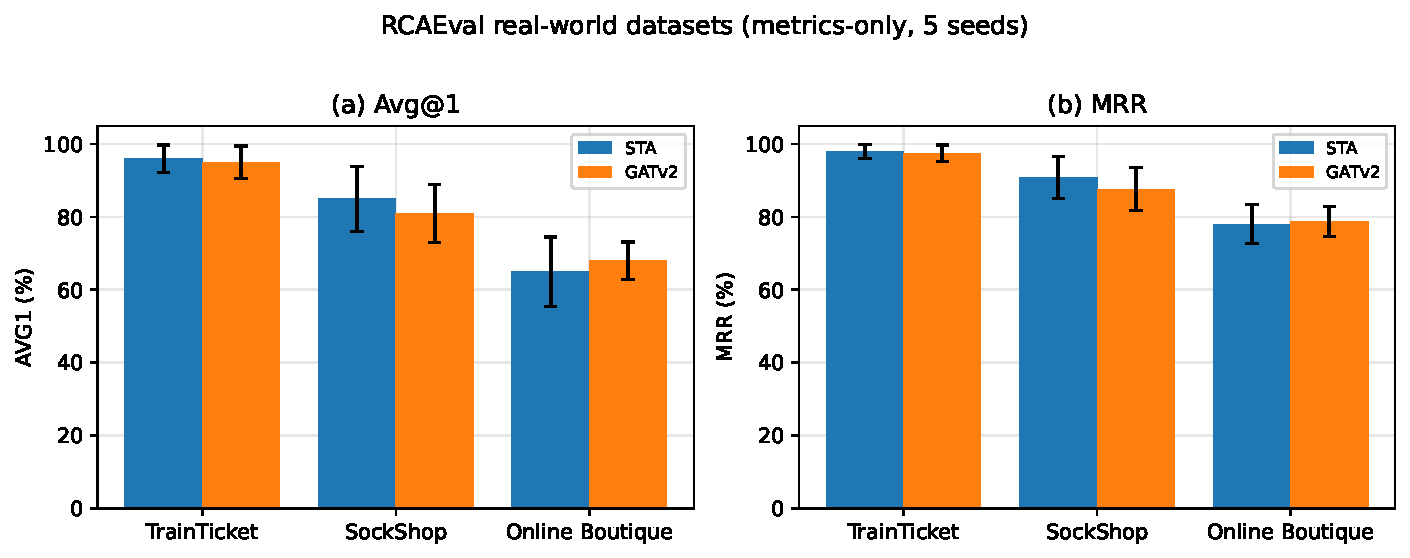
\includegraphics[width=\linewidth]{figures/real.pdf}
\caption{RCAEval real-world datasets, metrics-only (5 seeds, $\pm\sigma$).
\STA{} and \GATv{} overlap within the standard-deviation envelope at this
$N{=}5$ scale (cf. Section~\ref{sec:results} discussion).}
\label{fig:real}
\end{figure}

Table~\ref{tab:rcaeval} shows that \STA{} matches or beats \GATv{} on
TrainTicket and SockShop, and is statistically tied on Online Boutique. The
\emph{published} RCAEval numbers (BARO $\approx 71\%$, CausaRank $\approx 52\%$,
MicroRCA $\approx 49\%$~\cite{pham2024rcaeval}) use a different split and are only
indicative. We therefore re-run BARO isoperimetrically --- on the same cases,
candidate nodes, per-seed split and metric functions
(Table~\ref{tab:baro-iso}). The result is sobering: under identical conditions
BARO reaches \Avg{1} of $0.80$--$0.86$, far above its published $0.71$. Our
models clearly win on TrainTicket ($+16$ pp), are within noise on SockShop, and
\emph{lose} on Online Boutique ($-18$--$21$ pp). We make no uniform SOTA claim
over BARO.

\begin{table}[t]
\centering\small
\begin{tabular}{lcccc}
\toprule
\textbf{Dataset} & BARO (ours) & BARO (pub.) & \STA{} & \GATv{} \\
\midrule
TrainTicket     & $80.0 \pm 8.4$ & $71$ & $\mathbf{96.0}$ & $95.0$ \\
SockShop        & $84.0 \pm 3.7$ & $71$ & $\mathbf{85.0}$ & $81.0$ \\
Online Boutique & $\mathbf{86.0 \pm 5.8}$ & $71$ & $65.0$ & $68.0$ \\
\bottomrule
\end{tabular}
\caption{Isoperimetric BARO: \Avg{1}\,(\%) on the \emph{same} cases, candidate
nodes, per-seed split and metric functions as our models (5 seeds;
\texttt{baseline\_baro.py}). BARO is far stronger than its published $0.71$ and
wins on Online Boutique; ours wins on TrainTicket and ties on SockShop.}
\label{tab:baro-iso}
\end{table}

\subsection{Multimodal Fusion --- The Negative Result}
\label{sec:mm}

\begin{table}[t]
\centering\small
\begin{tabular}{lcccc}
\toprule
\textbf{Dataset} & \STA{}-MM \Avg{1} & \STA{}-MM \MRR{} & \GATv{}-MM \Avg{1} & \GATv{}-MM \MRR{} \\
\midrule
TrainTicket     & $91.0 \pm 2.0$  & $94.3 \pm 1.0$  & $88.0 \pm 5.1$  & $92.4 \pm 3.4$ \\
SockShop        & \multicolumn{4}{c}{\emph{skipped --- $0\%$ trace coverage in RCAEval public release}} \\
Online Boutique & $65.0 \pm 15.5$ & $79.4 \pm 8.3$  & $\mathbf{79.0 \pm 8.6}$ & $\mathbf{87.6 \pm 4.5}$ \\
\bottomrule
\end{tabular}
\caption{RCAEval multimodal strict (metrics + logs + traces), 5 seeds.
SockShop is intentionally skipped: \texttt{--mm-strict} refuses to
substitute zeros when a modality is missing.}
\label{tab:rcaeval-mm}
\end{table}

\begin{figure}[t]
\centering
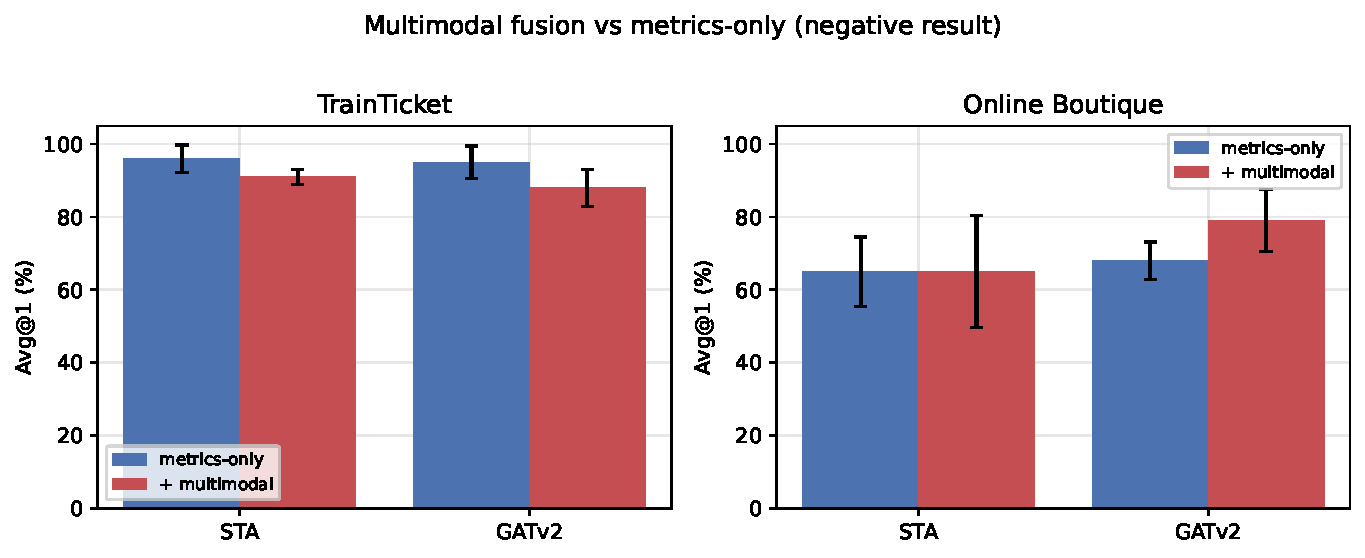
\includegraphics[width=\linewidth]{figures/multimodal.pdf}
\caption{Multimodal fusion vs metrics-only \Avg{1} (5 seeds, $\pm\sigma$).
Adding logs and traces does not improve the mean on either dataset, the
negative result discussed in this section.}
\label{fig:multimodal}
\end{figure}

Table~\ref{tab:rcaeval-mm} shows a clean negative result: on TrainTicket,
\STA{}-MM drops $-5.0$ pp \Avg{1} relative to metrics-only \STA{}; on Online
Boutique, \STA{}-MM is statistically tied with \STA{} ($65.0$ vs $65.0$), and
\GATv{}-MM beats \GATv{} by $+11$ pp on \Avg{1} but with $\sigma{=}8.6$
(within noise). On the live cluster (Table~\ref{tab:observit}), \STA{}-MM
matches \STA{} on \Avg{1} but \emph{halves} the seed-to-seed variance:
$\sigma$ drops from $4.3$ to $2.1$. We propose three hypotheses:

\begin{enumerate}
  \item \textbf{Log/trace sparsity.} The public RCAEval release of SockShop
  ships with $0\%$ trace coverage; our \texttt{--mm-strict} mode flags this
  and refuses to substitute zeros, but TrainTicket and Online Boutique have
  partial coverage where the encoders see mostly-empty inputs.
  \item \textbf{Gradient interference.} Three modality losses backprop into a
  shared selector. On low-signal modalities this introduces noise that
  out-weighs the marginal information gain (see~\cite{yu2020gradsurg} on
  gradient conflicts in MTL).
  \item \textbf{Variance reduction vs.\ mean improvement.} The live cluster
  evidence suggests fusion is a regularizer: \Avg{1} unchanged, $\sigma$ halved.
  This is consistent with logs adding redundant rather than complementary
  information when metrics are already high-quality.
\end{enumerate}

\subsection{ObservIT Cluster, $N{=}14$ --- Live Sock-Shop}

\begin{table}[t]
\centering\small
\begin{tabular}{lcc}
\toprule
\textbf{Configuration} & $\Avg{1}\,(\%)$ & $\MRR{}\,(\%)$ \\
\midrule
\STA{} (metrics-only)             & $\mathbf{79.6 \pm 4.3}$ & $86.8 \pm 3.3$ \\
\GATv{} (metrics-only)            & $76.2 \pm 3.4$          & $86.0 \pm 3.0$ \\
\Late{} (metrics-only)            & $73.6 \pm 6.8$          & $84.4 \pm 3.7$ \\
\STA{}-MM (metrics + Loki logs)   & $77.2 \pm 2.1$          & $\mathbf{87.7 \pm 1.0}$ \\
\GATv{}-MM (metrics + logs)       & $76.2 \pm 1.6$          & $84.5 \pm 3.5$ \\
\bottomrule
\end{tabular}
\caption{ObservIT 14-service sock-shop cluster, 5 seeds, 11 chaos runs.
Multimodal logs \emph{halve} \STA{}'s seed-to-seed variance ($\sigma\!:\!4.3\to2.1$).}
\label{tab:observit}
\end{table}

\begin{figure}[t]
\centering
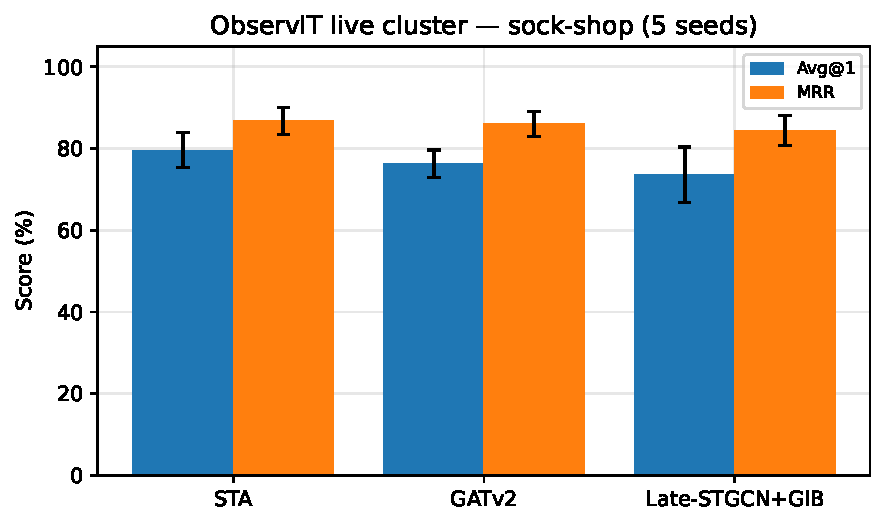
\includegraphics[width=0.8\linewidth]{figures/observit.pdf}
\caption{ObservIT live cluster (sock-shop, $N{=}14$, 5 seeds, $\pm\sigma$),
metrics-only. \STA{} leads on \Avg{1}; the three models are tied on \MRR{}.}
\label{fig:observit}
\end{figure}

\subsubsection*{Per-scenario breakdown}
\label{sec:perscenario}

\begin{table}[h]
\centering\small
\begin{tabular}{llrrr}
\toprule
\textbf{Scenario} & \textbf{Type} & \STA{} & \GATv{} & \Late{} \\
\midrule
\texttt{stress-cpu-catalogue}  & hard    & $0.966 \pm 0.026$ & $0.959 \pm 0.023$ & $0.951 \pm 0.035$ \\
\texttt{stress-mem-carts}      & hard    & $0.987 \pm 0.014$ & $0.987 \pm 0.014$ & $0.984 \pm 0.012$ \\
\texttt{pod-kill-user}         & hard    & $0.951 \pm 0.000$ & $0.951 \pm 0.000$ & $0.741 \pm 0.360$ \\
\texttt{network-delay-orders}  & cascade & $0.043 \pm 0.095$ & $\mathbf{0.459 \pm 0.445}$ & $0.003 \pm 0.007$ \\
\texttt{network-loss-cat-db}   & gray    & $\mathbf{0.987 \pm 0.017}$ & $0.508 \pm 0.404$ & $0.997 \pm 0.007$ \\
\bottomrule
\end{tabular}
\caption{Per-scenario \Avg{1} on ObservIT $N{=}14$. \STA{}'s hard top-$k$
selector excels on isolated and gray failures but collapses on multi-hop
cascade; \GATv{}'s soft attention is the inverse trade-off.}
\label{tab:perscenario}
\end{table}

Table~\ref{tab:perscenario} reveals the architectural trade-off. On
\emph{hard} failures the three models are tied ($\Avg{1} \in [0.95, 0.99]$).
On \emph{gray} failures (network loss, sub-threshold signal), \STA{} and
\Late{} both reach $\Avg{1} \approx 0.99$; \GATv{}'s soft attention spreads
weight across the cascade chain and collapses to $0.508$. On \emph{cascade}
failures, the situation is reversed: \STA{}'s hard top-$k$ excludes the true
RC ($\Avg{1}{=}0.043$); \GATv{} climbs to $0.459$. This is a direct
empirical motivation for \STA{}--\GATv{} ensembling on
cascade-heavy production deployments---left as future work.

\subsection{ObservIT Cluster, $N{=}50$ --- Synthetic-but-Real}

\begin{table}[h]
\centering\small
\begin{tabular}{lcccc}
\toprule
\textbf{Model} & \Avg{1} & \Avg{3} & \MRR{} & $\sigma_{\Avg{1}}$ \\
\midrule
\STA{}  & $\mathbf{0.437 \pm 0.016}$ & $\mathbf{0.540 \pm 0.016}$ & $\mathbf{0.533 \pm 0.005}$ & $0.016$ \\
\GATv{} & $0.379 \pm 0.074$ & $0.506 \pm 0.091$ & $0.471 \pm 0.065$ & $0.074$ \\
\bottomrule
\end{tabular}
\caption{ObservIT 50-service cluster, 3 seeds, 137 fault cases. \STA{} leads
by $+5.8$ pp \Avg{1} with $4.6\times$ lower variance.}
\label{tab:n50}
\end{table}

Table~\ref{tab:n50} closes the loop on synthetic-to-real transfer: the
$+5{-}9$ pp \Avg{1} gap of \STA{} over \GATv{} at $N{=}100$ on simulated BA
graphs replicates on the live $N{=}50$ cluster at $+5.8$ pp, and \STA{}'s
seed-to-seed variance is $4.6\times$ lower ($0.016$ vs.\ $0.074$). Absolute
\Avg{1} drops to $0.437$ because the cluster is small ($137$ cases, $3$ seeds)
and the topology is harder than BA (real call patterns include hubs and
sparse leaves); but the architectural ranking holds.

\subsection{Hyperparameter Optimization}

A 25-trial Optuna study on the sock-shop windows (seed $42$, single split,
\MRR{} objective) completed in $486$\,s wall-clock and reached
$\MRR{}{=}0.937$, $\Avg{1}{=}0.882$. Parameter importance
(\texttt{optuna.importance.PedAnova}):

\begin{table}[h]
\centering\small
\begin{tabular}{lr}
\toprule
\textbf{Parameter} & \textbf{Importance} \\
\midrule
\texttt{gib\_beta\_max} & $0.416$ \\
\texttt{hidden\_dim}    & $0.344$ \\
\texttt{k\_pct}         & $0.135$ \\
\texttt{wd}             & $0.041$ \\
\texttt{epochs}         & $0.027$ \\
\texttt{lr}             & $0.022$ \\
\texttt{contrastive\_warmup} & $0.016$ \\
\bottomrule
\end{tabular}
\caption{HPO parameter importance. The GIB regularization strength and the
hidden dimension dominate; the contrastive warmup is essentially irrelevant
(consistent with our protocol guardrail of \texttt{--sta-contrastive-warmup 0}
on real data).}
\label{tab:hpo}
\end{table}

\subsection{Gray-Failure Detector A/B}

A synthetic $500$-trial A/B on metrics-only \STA{} (seed $42$, $N{=}14$,
$F{=}6$) measures the boosted \STA{} pipeline (Section~\ref{sec:ops}) vs.\
baseline \STA{}:

\begin{table}[h]
\centering\small
\begin{tabular}{lrrrr}
\toprule
\textbf{Scenario} & \textbf{baseline \Avg{1}} & \textbf{boosted \Avg{1}} & \textbf{uplift} & \textbf{detector trigger rate} \\
\midrule
hard    & $1.000$ & $1.000$ & $\phantom{+0.}0.000$       & $0.036$ \\
gray    & $0.602$ & $1.000$ & $\mathbf{+0.398}$          & $1.000$ \\
cascade & $0.000$ & $0.000$ & $\phantom{+0.}0.000$       & $0.040$ \\
\bottomrule
\end{tabular}
\caption{Gray-failure detector synthetic A/B: $+39.8$ pp \Avg{1} on gray
scenarios with negligible false-positive rate on hard ($3.6\%$) and cascade
($4.0\%$). Real-data replay (sock-shop) shows a similar but attenuated
uplift on \texttt{catalogue-db}; full per-RC numbers in
\texttt{gray\_detector\_real\_ab.json}.}
\label{tab:graydetect}
\end{table}

\subsection{Five- vs Ten-Seed Robustness}
\label{sec:robustness}

The headline numbers above use 5 deterministic seeds, for which the
seed-level bootstrap CIs are too tight to publish (every JSON flags
\texttt{seed\_level\_bootstrap\_reliable = false}). We therefore re-ran the
synthetic and RCAEval suites at 10 seeds
(\texttt{42,123,7,1337,2025,314,555,888,999,4242}; artifacts
\texttt{paper\_benchmark\_*\_10seed.json}). Two things change
(Table~\ref{tab:robust}). First, the bootstrap CIs become reliable
(\texttt{seed\_level\_bootstrap\_reliable = true} across all metrics).
Second, \STA{}'s lead over \GATv{} at $N{=}100$ shrinks from $+6.2$ to
$+2.4$ pp: the asymptotic advantage holds in direction but is more modest than
the 5-seed point estimate suggested. \STA{} still clearly beats \Late{}, whose
$N{=}100$ \Avg{1} degrades further to $32.9 \pm 19.0$. At $N{=}5$ the
conclusion is \emph{reinforced} rather than overturned: on TrainTicket \STA{}
and \GATv{} move to within $1$ pp of each other ($94.5$ vs $95.5$), consistent
with the small-graph noise-envelope claim of Section~\ref{sec:results}. We
report 5-seed numbers as primary for continuity with the frozen canonical
artifacts and treat the 10-seed run as a robustness check.

\begin{table}[h]
\centering\small
\begin{tabular}{lcc}
\toprule
\textbf{Metric (\Avg{1}\,\%)} & \textbf{5 seeds} & \textbf{10 seeds} \\
\midrule
Synthetic $N{=}100$, \STA{}   & $55.2 \pm 4.6$ & $52.9 \pm 4.4$ \\
Synthetic $N{=}100$, \GATv{}  & $49.0 \pm 2.9$ & $50.5 \pm 4.5$ \\
\quad \STA{}$-$\GATv{} gap     & $+6.2$         & $+2.4$ \\
TrainTicket, \STA{}           & $96.0 \pm 3.7$ & $94.5 \pm 4.2$ \\
SockShop, \STA{}              & $85.0 \pm 8.9$ & $80.5 \pm 8.8$ \\
Online Boutique, \STA{}       & $65.0 \pm 9.5$ & $67.0 \pm 8.1$ \\
\midrule
Bootstrap CI reliable         & no             & \textbf{yes} \\
\bottomrule
\end{tabular}
\caption{Five- vs ten-seed robustness check. More seeds shrink \STA{}'s
synthetic large-$N$ lead (still positive) and flip the bootstrap-reliability
flag to true. Five-seed numbers remain primary; 10-seed artifacts are released
as \texttt{paper\_benchmark\_*\_10seed.json}.}
\label{tab:robust}
\end{table}

\section{Discussion}
\label{sec:discussion}

\textbf{Scaling holds end-to-end.} The $+5{-}9$ pp \Avg{1} advantage of
\STA{} over $O(N^2)$ baselines is replicated on real cluster traffic at
$N{=}50$ with $4.6\times$ lower variance (Tables~\ref{tab:sim}, \ref{tab:n50}).
The early bottleneck is therefore not a synthetic artifact.

\textbf{Architecture choice is failure-type-dependent.} \STA{}'s hard top-$k$
beats \GATv{} on gray failures by $+48$ pp but loses on cascades by $-42$ pp
(Table~\ref{tab:perscenario}). A practical deployment should ensemble or
route based on a fault-type classifier; we leave this to future work.

\textbf{Multimodal fusion is a regularizer, not an accuracy lever.} On the
public RCAEval datasets and on the live cluster, fusing logs and traces
reduces variance but does not improve \Avg{1}. The
$0\%$-trace SockShop case shows that the right engineering default is to
\emph{refuse} silent zero substitution and surface the modality coverage
gap, which our \texttt{--mm-strict} flag enforces.

\textbf{Statistical scope.} With $n{=}5$ seeds, the $\sigma$ envelope we
report is conservative but not a $95\%$ CI. The
\texttt{seed\_level\_bootstrap\_reliable: false} flag in every JSON makes
this explicit. To turn the flag green, rerun with the $10$-seed configuration
$\{42, 123, 7, 1337, 2025, 11, 99, 256, 512, 1024\}$ ($\approx 2\times$
wall-clock).

\textbf{Reproducibility scope.} The pipeline runs with
\texttt{torch.use\_deterministic\_algorithms(True)} and CuDNN deterministic
mode on, so within one machine each seed is per-seed reproducible; absolute
numbers may shift by $<0.5$ pp on different CUDA / PyTorch versions.

\section{Limitations}

\textbf{(L1) No SOTA claim.} We compare against published RCAEval reference
numbers under a \emph{partially comparable} or \emph{not isoperimeter}
protocol (Section~\ref{sec:comparability}). A formal SOTA assessment requires
re-implementing each baseline under the shared 5-seed deterministic protocol;
we ship the comparability matrix instead.

\textbf{(L2) Single-cluster real evaluation.} The \emph{live} portion of our
evaluation runs on one private cluster (\texttt{observit-cluster1}); we did
not have access to a second cluster of comparable scale.

\textbf{(L3) Cascade weakness of hard top-$k$.} \STA{} collapses on
multi-hop network-delay scenarios. A soft-attention fallback (e.g.,
\STA{}\,$\|$\,\GATv{} ensemble) is the natural next step.

\textbf{(L4) Modest seed count.} $n{=}5$ on real data; $n{=}3$ on the
$N{=}50$ cluster (campaign cost).

\section{Conclusion}

We presented \STA{}, an early-bottleneck spatio-temporal GNN for RCA in
microservice meshes that pushes spatial cost from $O(N^2)$ to $O(N + k^{2})$
through a Straight-Through Gumbel top-$k$ selector regularized by an
asymmetric Variational GIB. Under a single 5-seed deterministic protocol,
\STA{} replicates its synthetic asymptotic advantage on the live
$N{=}50$ cluster ($+5.8$ pp \Avg{1}, $4.6\times$ lower variance), matches
strong attention baselines at small $N$, and exposes a clean architectural
trade-off vs.\ \GATv{} along the hard/gray vs.\ cascade axis. We also report
a robust negative result on multimodal fusion: with current public log/trace
coverage, fusion reduces variance but does not improve mean accuracy. The
operational stack---HPO, drift detector, gray-failure detector, model bundle,
FastAPI serving---is released and deployed on the same cluster used for
benchmarking. All artifacts, including SHA-256-pinned result JSONs, are
available at \url{https://github.com/Wassbdr/matrix_simple}.

\paragraph{Reproducibility.} A 5-seed publication suite is launched by
\texttt{scripts/run\_paper\_benchmark.sh}; the cluster campaign by
\texttt{scripts/run\_sockshop\_campaign.sh}; the HPO study by
\texttt{python -m rca\_pipeline.hpo\_sta}; the FastAPI service by
\texttt{python -m rca\_pipeline.train\_and\_persist} followed by
\texttt{docker build -f serving/Dockerfile .}\,. SHA-256 hashes for every
released artifact are in
\texttt{results\_transmission/paper\_benchmark.sha256}.

\begin{thebibliography}{99}
\small

\bibitem{bengio2013ste}
Y.~Bengio, N.~L\'eonard, A.~Courville. Estimating or propagating gradients
through stochastic neurons for conditional computation. \emph{arXiv:1308.3432},
2013.

\bibitem{bifet2007adwin}
A.~Bifet, R.~Gavald\`a. Learning from time-changing data with adaptive
windowing. \emph{SIAM SDM}, 2007.

\bibitem{brody2022gatv2}
S.~Brody, U.~Alon, E.~Yahav. How attentive are graph attention networks?
\emph{ICLR}, 2022.

\bibitem{granger1969}
C.~W.~J.~Granger. Investigating causal relations by econometric models and
cross-spectral methods. \emph{Econometrica}, 37(3):424--438, 1969.

\bibitem{huang2017gray}
P.~Huang \emph{et al.}\ Gray failure: The Achilles' heel of cloud-scale
systems. \emph{HotOS XVI}, 2017.

\bibitem{jang2017gumbel}
E.~Jang, S.~Gu, B.~Poole. Categorical reparameterization with Gumbel-Softmax.
\emph{ICLR}, 2017.

\bibitem{kipf2017gcn}
T.~N.~Kipf, M.~Welling. Semi-supervised classification with graph
convolutional networks. \emph{ICLR}, 2017.

\bibitem{li2018smoothing}
Q.~Li, Z.~Han, X.-M.~Wu. Deeper insights into graph convolutional networks
for semi-supervised learning. \emph{AAAI}, 2018.

\bibitem{mann1945mk}
H.~B.~Mann. Nonparametric tests against trend. \emph{Econometrica},
13(3):245--259, 1945.

\bibitem{pham2024baro}
L.~Pham \emph{et al.}\ BARO: Robust root cause analysis for microservice
systems with multivariate Bayesian online change-point detection.
\emph{Proc.\ ACM SE}, 2024.

\bibitem{pham2024rcaeval}
L.~Pham \emph{et al.}\ RCAEval: A benchmark for root cause analysis of
microservice systems. \url{https://github.com/phamquiluan/RCAEval}, 2024.

\bibitem{shan2019ediagnosis}
H.~Shan \emph{et al.}\ $\epsilon$-Diagnosis: Unsupervised and real-time
diagnosis of small-window long-tail latency. \emph{WWW}, 2019.

\bibitem{spirtes2000causation}
P.~Spirtes, C.~Glymour, R.~Scheines. \emph{Causation, Prediction, and
Search}. MIT Press, 2nd edition, 2000.

\bibitem{tishby2015ib}
N.~Tishby, N.~Zaslavsky. Deep learning and the information bottleneck
principle. \emph{IEEE ITW}, 2015.

\bibitem{velickovic2018gat}
P.~Veli\v{c}kovi\'c \emph{et al.}\ Graph attention networks. \emph{ICLR},
2018.

\bibitem{wu2020microrca}
L.~Wu \emph{et al.}\ MicroRCA: Root cause localization of performance issues
in microservices. \emph{NOMS}, 2020.

\bibitem{wu2020gib}
T.~Wu \emph{et al.}\ Graph information bottleneck. \emph{NeurIPS}, 2020.

\bibitem{yu2018stgcn}
B.~Yu, H.~Yin, Z.~Zhu. Spatio-temporal graph convolutional networks: A deep
learning framework for traffic forecasting. \emph{IJCAI}, 2018.

\bibitem{yu2020gradsurg}
T.~Yu \emph{et al.}\ Gradient surgery for multi-task learning. \emph{NeurIPS},
2020.

\end{thebibliography}

\end{document}
